\chapter{Experiments With Real Multi-copters}

As a final step the algorithms were tested using two high-end quadcopters available in the laboratory. In particular the multi-copters are produced by Ascending Technologies and are:
\begin{itemize}
\item Asctec Firefly (hexacopter)
\item Asctec Pelican (quadcopter)
\end{itemize}

\begin{figure}[H] 
  \begin{minipage}[b]{0.5\linewidth}
    \centering
    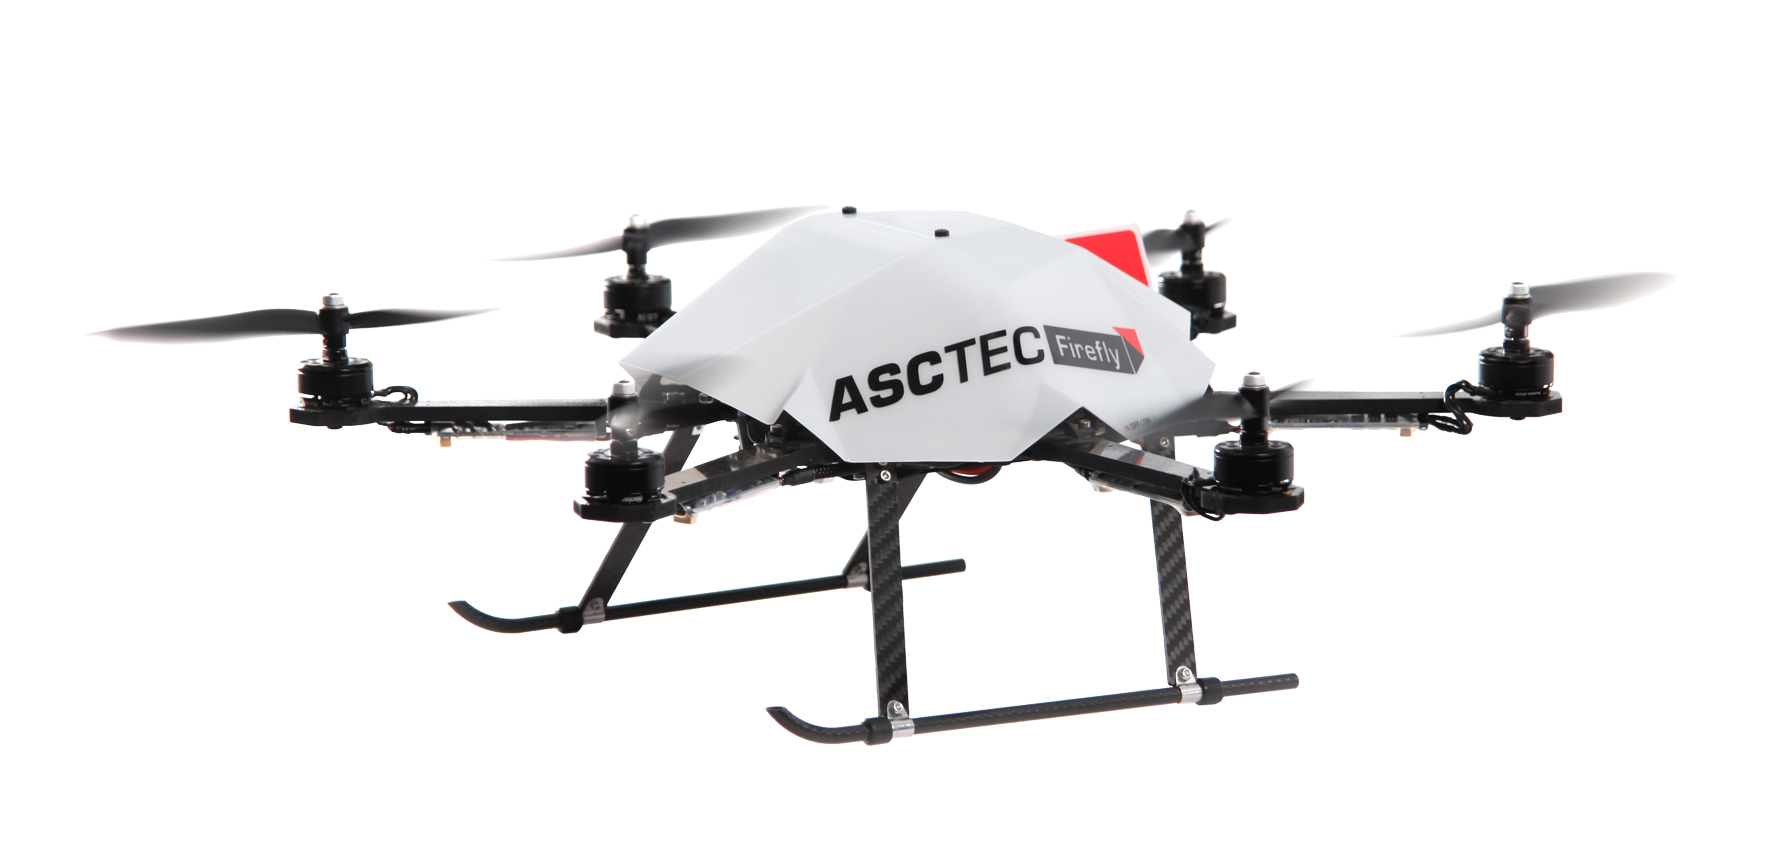
\includegraphics[width=0.8\textwidth]{asctec_firefly}
    \caption{Asctec Firefly}
    \label{fig:firefly}
    \vspace{4ex}
  \end{minipage}
  \begin{minipage}[b]{0.5\linewidth}
    \centering
    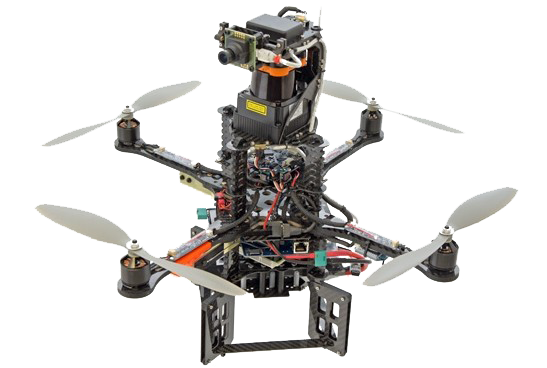
\includegraphics[width=0.7\textwidth]{asctec_pelican}
    \caption{Asctec Pelican}
    \label{fig:pelican}
    \vspace{4ex}%%
  \end{minipage}
\end{figure}


They both mount an on-board computer which runs Linux and Wi-Fi adapter through which is performed all the communication. For the robot dynamic control system the ETHNOS \cite{ethnos2000} real-time software framework is used. The ETHNOS environment is composed of a dedicated distributed real-time operating system (developed as an extension to Linux), from which the overall environment takes its name, with a dedicated network protocol designed for both the single robot and the multi-robot environment, specifically designed for noisy wireless communication. Using a dedicated ROS/ETHNOS interface the communication between the path planner and the controller is made possible.


\section{Multi-rotor model and parameters tuning}


During the experiments ``on the field'' the main part was spent in the fine tuning of the quadcopters controllers. In particular by adjusting the PID parameters that control the propellers thrust in reaching a given target. In this section we will give a general idea of the control scheme and how this applies to the quadcopter dynamics.

To describe the ideal dynamics of a multi-rotor aircraft we can use the following mathematical model \cite{2010JSDD4255A}:

\begin{equation}
  \begin{cases}
   \ddot{\xi} = \frac{1}{m}uR{e_3}-g{e_3} \\
   M(\eta)\ddot{\eta}+C(\eta,\dot{\eta})\dot{\eta} = \Uppsi(\eta)^{T}\tau
  \end{cases}
\end{equation}

where $m,\xi$ and $\eta$ are the aircraft mass, position and orientation respectively. $(u, \tau)$ are the applied thrust and torque vector, $R$ and $\Uppsi$ are the rotation matrix and Euler matrix respectively. \\% The pseudo inertial matrix $M$ is defined as $M(\eta) = \Uppsi(\eta)^{T}J\Uppsi(\eta)$, and the centripetal vector C is given by \mbox{$C(\eta,\dot{\eta}) =  \Uppsi(\eta)^{T}J\dot{\Uppsi}(\eta)-\Uppsi(\eta)^{T}sk(\Uppsi(\eta)\dot{\eta})J\Uppsi(\eta)$}.
For autonomous multi-rotors it is common to separate the flight control problem into an ``inner-loop'' that controls attitude and an ``outer-loop'' that controls the translational trajectory of the aircraft. After transforming the original system into one that describes the position dynamics \cite{kendoul:hal-00338358} we can finally the PID controller as follows:

\begin{equation}
\mu{_x} = - K_{P_x}(x - x_d) - K_{I_x} \int (x - x_d) dt - K_{D_x}(v_x-v_{x}d)
\end{equation}

And the same goes for $y$ and $z$. This is the so called outer-loop position control. $\mu$ is an intermediate control vector and after evaluating $\mu{_x}$, $\mu{_y}$ and $\mu{_z}$ we can calculate the desired thrust $u$, roll angle $\phi_d$ and pitch angle $\theta_d$ that  constitutes the input parameters for the inner-loop , the \emph{attitude controller}:

\begin{equation}
  \begin{cases}
   u = m \sqrt{{\mu{_x}}^2 + {\mu{_y}}^2 + {(\mu{_z}+g)}^2} \\
  \phi_d = sin^{-1} \left( m\dfrac{ \mu{_x} sin\psi_d - \mu{_y} cos\psi_d }{ u } \right) \\
  \theta_d = tan^{-1} \left( \dfrac{ \mu{_x} cos\psi_d - \mu{_y} sin\psi_d }{ \mu{_x} + g} \right)
  \end{cases}
\end{equation}

where $g$ is the gravity acceleration that has to be compensated to fly and $\psi_d$ is the yaw angle which represent the aircraft heading direction. In general $\psi_d$ can be set to zero, as the orientation of the multi-rotor is not relevant unless it mounts some front directional camera. The attitude controller will then care of transforming these values into input controls for the aircraft's propellers. The standard PID controller can be represented using a block diagram as in figure \ref{fig:pid_blockDiag}.

\begin{figure}[h]
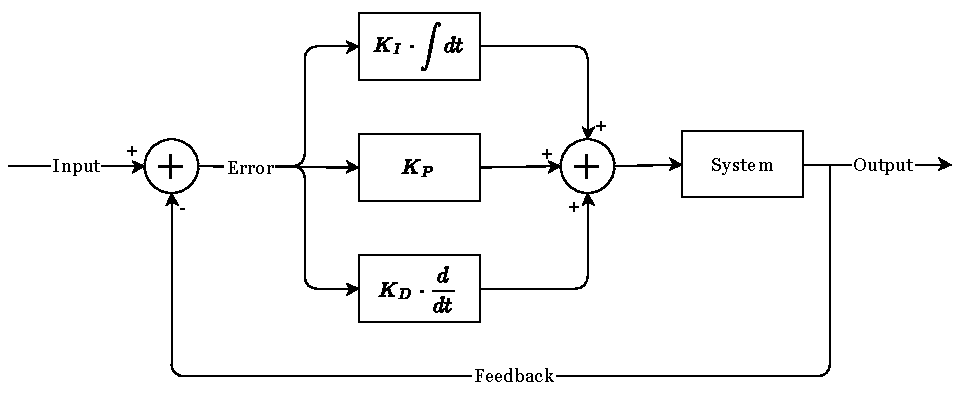
\includegraphics[width=\textwidth]{pid_controller}
\caption{A general PID controller block diagram}
\label{fig:pid_blockDiag}
\end{figure}


To have any kind of control over the quadcopter or multi-copter, we need to be able to measure the quadcopter sensor output (for example the pitch angle), so we can estimate the error (how far we are from the the desired pitch angle, e.g. horizontal, 0 degree). We can then apply the 3 proportional (P), integrative (I) and derivative (D) control algorithms to the error, to get the next outputs for the motors aiming to correct the error.

The three parameters that we can adjust to improve better quadcopter stability are the $K_P$, $K_I$, $K_D$ gains showed in figure \ref{fig:pid_blockDiag}. Each gain coefficent basically would change the importance and influence of each algorithm to the output. Let's now look at what are the effects of these parameters to the stability of a quadcopter.


Since we want to control the quadcopter's $(x,y,z)$ position in space, the parameters will be described in terms of how they affect the process of keeping the desired position.

The proportional gain coefficient $K_P$ determines how fast the quadcopter will reach the desired position. The higher the coefficient, the higher the multi-copter will be sensitive and reactive to position change. If it is too low, the quadcopter will appear sluggish and will be harder to keep steady. If the P gain is too high the multi-copter may start to oscillate with a high frequency and overshoot the target repeatedly. %
The integral gain coefficient $K_I$ can increase the precision of the final position since it will eliminate the so called \emph{steady-state error}. This term is especially useful with irregular wind, and ground effect (turbulence from motors). However, when the $K_I$ value gets too high your quadcopter might begin to have slow reaction and a decrease effect of the proportional gain as consequence, it will also start to oscillate like having high $K_P$ gain, but with a lower frequency. %
The derivative gain coefficient $K_D$ will impact what the other two gain cannot control that is reduce the overshoot and the settling time. It will also work like a damping factor against the previous two, to prevent excessive oscillation in a situation of high $K_P$ and $K_I$. It  This parameter is extremely delicate since it depends on the rate of change of the error and in certain cases it may amplify the effects of the previous gains.  %

Since finding the exact parameters of the mathematical model of each quadcopter can be extremely difficult the most common way to tune this parameters is by trial and error. In the following paragraph there are a couple rules of thumb. To tune quadcopter $K_P$ gain the procedure is to slowly increase it until the quadcopter reaches the position without producing big oscillations. For the $K_I$ gain, again start low and increase slowly, paying attention to how long does it take to stop and stabilize. You want to get to a point where it stabilize very quickly while not wandering around for too long. To get a reliable I-value a test under windy condition may be useful. For $K_D$ gain, it can get into a complicated interaction with $K_P$ and $K_I$ values. When using D gain, you need to go back and fine tune P and I to keep the plant well stabilized.

\section{Results}
Here we present the results for the Node Counting algorithm



